% Copyright (c) 2014,2016 Casper Ti. Vector
% Public domain.

\chapter{数据与模型设计}

\section{数据处理}

\subsection{tex文件到图片}
\noindent

我们首先从网上获得了大量的论文Tex文件。Tex语法中行内公式有明确的标注,通过正则表达式找到其中被\$...\$框住的公式部分,由于我们的关注点只在于行内公式,故被\$\$...\$\$框住的行间公式部分需要排除,找到后在公式外加上可以框住公式的LaTeX 命令,并分为使用红框和使用白框两个版本。使用白框的是我们进行训练的主要数据,红框版本是获得标记使用的。为了支持我们新增的LaTeX命令,仍需要使用正则表达式检测是否含有我们需要的宏包,若没有则在开头加上。接着将处理完毕的Tex文件编译为PDF文件,在编译过程中发现大量的编译失败,主要原因一是使用的Tex文件较为久远,主要为2001-2003年的数据,编译格式和使用的宏包各种各样或已淘汰,缺少相应的宏包支持,二是有的文件的编码格式不是utf-8,而编译时统一以utf-8为标准,故导致了读取失败。成功编译的PDF中也有少量缺失正文,只有公式存在。而且由于为了迅速编译,故所有文件只进行了一次编译,这样所有的参考文献引用都不会生效,参考文献的编号都变成了?,认为不影响本工作,所以忽略该问题。

然后是将PDF文件转化为png图片。由于预计使用工具magick来进行转化,而为了全程使用python编程,故使用了magick的python包PythonMagick,而此包缺少文档说明,故一开始转化为png时遇到了困难,故使用的是jpg格式,这样输出的图片数据占用比较大。在查阅了许多解决方法后才终于得到了png文件,发现相同尺寸下png格式的图片只有jpg格式的几分之一,大大减小了硬盘占用,加快了数据传输与处理。

以上方法都写在了文件texf\_topng.py中。宏包使用了re, os, pdflatex, PythonMagick, PyPDF2, 并导入了自己写的图片处理工具文件。re为使用正则表达式的宏包,pdflatex是将tex编译为pdf的宏包,PythonMagick是将pdf转化为png的宏包,PyPDF2是辅助pdf分页生成图片的宏包。在生成图片的同时裁去了图片的空白边框并通过生成的图片是否有红框来删去了不带公式的图片,以减少不必要的数据。单个tex文件处理使用文件ttp.py,批量文件处理使用ttpb.py。通过以上方法生成了红框版本和白框版本共计16万张图片,每张图片的生成速度在一秒以内,实际生成时使用并行处理。本方法由于还要将论文图片分割为单词,故实际使用的图片数没有这么多。

\subsection{单词分割及数据预处理}
\noindent

单词分割主要分为两个部分,文行分割与行内单词分割。图片的一行通常指图像矩阵的一行数据,故将文本中的一行称为文行。以下处理均使用灰度图像。行和是指图像矩阵一行中非空白元素的比例,由于提前做了图像反转,白色为0,黑色非零,故只需要将一行二值化后求和除以列数,故称为行和。文行的中心行和指文行中间一行的行和,同理,开始行和与结尾行和指文行开始行与结尾行的行和。

在处理之前首先判断图片方向,认为一般只有正向和逆时针90度方向。由于灰度图像白色为255,黑色为0,故先将图片矩阵反转为白色为0,黑色为255,再分别求得图片矩阵的行和和列和。如果图象是正向的,空白边框也已经被截去,故认为行和中0的比例应大于列和中0的比例,因文行和文行之间有固定的空白,而单词与单词之间的空白位置每行不一。以此作为是否要将图片旋转的依据。此判断只对整页文本图片有效果,若进行单行或单个单词测试则无效,故设置为可以关闭。

文行分割这个问题上,文行与文行之间有明显的空行,以空行作为文行的边界即可。由于只关心行内公式,故文行分割还有更多的要求,需要在分割时排除行间公式和一些特殊的文行,如一条直线、图表、页码、特殊符号等。故以空行作为边界分割后,又以中心行和,前四分之一行和,开始行和,结尾行和和行高度作为标准来去掉不符合需求的文行。行间公式和一条直线这种情况,一般高度与正常的文行有差别,行间公式大部分高度比较大,一条直线、特殊符号等则是高度比较小,故筛选出高度在平均高度一定范围内的文行。而页码则是中心行和极小,实际上行间公式的中心行和也小于正常文行的中心行和。同时行间公式的前面通常是一片空白,故同时使用前四分之一中心行和来同时作为辅助标准。开始行和和结尾行和则是为了去掉图表。在文行分割上如果出现更多的特殊情况还需要更多的标准,这里只写出了我实际遇到的问题。

文行分割后,就是对每一文行进行单词分割了,我们使用的都是英文文档,故这里只考虑英文的单词分割。同样预先进行图像反转,使得白色为0,黑色非零。单词分割与文行分割有相似之处,同样是利用单词与单词之间的空白。但容易注意到一行内的空白有三种情况,单词与单词间的空白、字母与字母间的空白和另外一些比较大的空白,如一行结尾后还有大片空白,每段开始文行的开头空白等。这些空白的位置使用列和就可以轻易找到,接下来就是在这些空白中筛选出单词间空白。由于最后是利用空白的位置来分割出单词,故认为大片空白和单词间空白是同一性质。这里使用的是最小二乘法,通过公式(2.1)获得使得$S(w)$最小的宽度$w$,然后认为在这宽度以上的都是用来分割单词的空白。这样做的效果还不错,大多数单词都可以分割出来,少数情况下会出现一个单词被分为两个,而常见的情况是一个长公式被分割为多个单词。

\begin{align}
    S(w) = \sum^n_{i=1} (w_i - w)^2
\end{align}

以上单词分割不仅可以分割出单词图片,同时可以获得分割出的文行的位置和每个文行中每个单词的位置,结合去除空白边框时获得的左上角的非空白元素的位置,可以将每个单词的位置精确地还原。

将白框版本的图片进行了单词分割,获得了单词图片及其位置,在通过其位置信息在红框版本的图片中检查该单词是否被红框框住,以此获得每个单词的标注。这样我们将原本的图片整理成了单词图片、单词位置信息和单词标注信息,训练神经网络只需要单词图片和标注信息,故将这部分做成tfrecords文件以备后续使用。由于一张论文图片中非公式单词比公式单词要多得多,故这里采用了过采样,将公式图片直接复数拷贝,使得公式图片与非公式图片的数量接近。过采样后实际使用的单词图片为100万张左右。

\section{网络结构与算法}

\subsection{激活函数与损失函数}
\noindent

神经网络中有两个重要的部分,一个是激活函数,一个是损失函数。激活函数是实现网络非线性化的重要手段,常用的激活函数有sigmoid函数、tanh函数和ReLu函数(2.2)等。其中sigmoid函数和tanh函数由于当输入比较大时会有梯度接近0的问题,即梯度消失,使得非监督训练的效果较差。
\begin{align}
    relu(x) = \begin{cases} 0& x < 0 \\ x& x \ge 0 \end{cases}
\end{align}
ReLu有计算简单迅速而且不会有梯度消失问题的优势。ReLu仍有些问题,一是若训练发散,会迅速增大或减少到nan,使得结果报错。故开始训练前应仔细检查网络的设置,确保能够收敛。二是ReLu函数将小于零的值直接变为0,使得该输出都为正值,故可能会造成某些神经元的失活,不管怎样训练都为0。同时ReLu的输出都为正值,使得收敛比较困难。故针对ReLu有许多的改进的函数。Leaky ReLu函数为在ReLu的基础上,在$x<0$时加上一个较小的斜率。PReLu则是使得这个斜率作为一个可以训练的参数加入网络中,RReLu的做法则是将这个斜率根据均匀分布随机抽取。PReLu的输出更近接近0,收敛速度比ReLu更快,故我使用的是PReLu。

分类问题使用的最普遍的的损失函数是交叉熵函数(2.3)
\begin{align}
    H(p, q) = - \sum_x p(x) \log q(x)
\end{align}
要使用交叉熵函数需要输出和目标都满足概率分布,故交叉熵函数一般结合softmax函数(2.4)将输出和目标都归一化。
\begin{align}
    softmax(y)_i = y'_i = \frac{e^{y_i}}{\sum^n_{j=1} e^{y_j}}
\end{align}
在二分类时也可以使用sigmoid函数(2.5)将输出转化到$[0, 1]$之间满足概率分布。
\begin{align}
    sigmoid(y) = \frac 1 {1 + e^{-y}}
\end{align}
在二分类时,softmax的表达式为
\begin{align}
    softmax(y)_1 = \frac{e^{y_1}}{e^{y_1} + e^{y_2}} = \frac 1 {1 + e^{y_2 - y_1}}
\end{align}
故神经网络输出的两个值的差与只输出一个值是等价的,差别在于前者的全连接层会有更多的训练参数。这里实际使用的是sigmoid函数。

\subsection{神经网络优化算法}

\subsubsection{指数衰减学习率}
\noindent

神经网络的学习率代表神经网络参数的更新速度,较大的学习率使得参数每次更新的幅度较大,收敛得更快,但可能会导致无法收敛到最小,每次更新的时候都跳过了能够收敛到最小值的范围;学习率太小又会导致参数更新太慢,网络收敛速度太小。一般而言,开始时希望学习率比较大,使得网络快速收敛,然后学习率逐渐降低,使得收敛更为准确。故使用了阶梯状指数衰减学习率(2.7),将学习率乘上一个指数衰减率,使得学习率随着训练次数逐渐降低。$\eta_0$为初始学习率,$\delta$为衰减系数,$s$为训练次数,$s_d$为衰减速度。即每经过$s_d$次训练,学习率会以$\delta$的比例衰减。实际为每学习1000轮将学习率乘以0.9。
\begin{align}
    \eta = \eta_0 \delta^{\lfloor s / s_d \rfloor}
\end{align}

\subsubsection{批标准化batch normalization}
\noindent

神经网络中的数据在经过每层的处理后数据分布可能会发生变化,这一过程被称为Internal Covariate Shift\parencite{bn}。这种数据分布的变化传递到后层网络中,后层网络也需要不停地去适应这种分布的变化,这就导致了网络的收敛速度下降。如果采用的是饱和激活函数,如sigmoid或tanh,数据分布变化会导致数据变大进入梯度饱和。而如果是ReLu激活函数,则会有数据分布差异大,深层网络收敛困难的问题\parencite{bn-relu}。

由于以上问题,我们使用了batch normalization方法,即对每层的数据做规范化。对一层中的一批数据的每个通道$\{x_i : 0 \le i \le n\}$,做如下规范化操作
\begin{align}
    &\mu = \frac 1 n \sum^n_{i = 1} x_i \\
    &\sigma^2 = \frac 1 n \sum^n_{i=1}(x_i - \mu)^2 \\
    &\hat{x}_i = \frac{x_i - \mu}{\sqrt{\sigma^2 + \varepsilon}}
\end{align}
$\varepsilon$是为了处理方差为0的特殊情况。这样规范化后每一层网络的数据分布都变得稳定,但数据的表达能力却缺失了。为了获得原有信息,BN又引进了两个可以在网络中进行学习的参数$\gamma$和$\beta$,使得规范化后的数据可以通过变换(2.11)恢复表达能力。
\begin{align}
    \tilde{x}_i = \gamma \hat{x}_i + \beta
\end{align}
当$\gamma^2 = \sigma^2, \beta = \mu$时,$\tilde{x}_i = x_i$,即是完全恢复为原来的数据。这样我们既使得每层的分布变得稳定,又能够保证数据的表达能力。规范化是在一个batch的每个通道上做,而偏置项对于一个通道而言是相同的,故只需要对卷积输出做规范化,然后加上偏置项就可以了。

BN使得网络的每层数据的分布变得稳定,后层网络不必去适应输入的变化,实现了每层的独立学习,提高了整个网络的学习速度。在使用ReLu激活函数时,由于ReLu函数的输出都非负,故输出平均值远离0,网络不容易收敛,若不使用BN,使用MSRA初始化30层以上的网络也难以收敛\parencite{bn-relu}。同时BN处理后,将降低网络中的参数的敏感度,使得调参,如初始化、学习率等的设置更为容易,不用担心参数的变化随着网络层数加深被放大。使用BN后,也不用担心数据经过多层网络后落入饱和性激活函数的梯度包和区,从而可以缓解使用sigmoid,tanh等激活函数的梯度消失问题。同时BN并没有完全保留原始数据的信息,而是通过学习参数$\gamma, \beta$来一定程度上保留数据的表达能力,这就相当于给数据加入了随机噪音,可以起到正则化的效果,防止数据的过拟合。在原作者的结果中,BN可以在没有dropout的情况下同样达到很好的泛化效果,而且网络的收敛速度提高了很多。\parencite{bn}我在网络中也同样使用了BN。

\subsubsection{滑动平均}
\noindent

滑动平均,或指数加权平均是一个使得神经网络模型在测试数据上更加健壮(robust)的方法,在计算网络输出时,使用的网络模型不是当时的模型,而与一段时间内的历史模型有关。变量$v_t$在更新为$t$时刻的取值$\theta_t$时,使用公式(2.12)
\begin{align}
    v_t = \beta v_{t-1} + (1 - \beta) \theta_t
\end{align}
上式中$\beta \in [0, 1)$,$\beta$一般取值较大,即变量在更新时使用了上一时刻的取值,做了某种平均,这样不需要保存一段时间内的每个网络就可以获得某种网络的均值。在网络训练的后期,网络会在在一定范围内波动,使用滑动平均后的网络变量来测试数据就能提高测试结果的表现和稳定性。注意到在网络训练的前期我们希望模型可以更新得更快,故希望衰减率较小,来使得变量快速学习更新。Tensorflow提供了tf.train.Exponential- movingAverage函数来实现滑动平均,还提供了参数num\_updates来实现动态设置衰减率的大小,使得网络前期衰减率较小,可以快速学习更新,训练到一定程度后则使用较大的衰减率来实现更好的滑动平均。

\subsubsection{过拟合优化}
\noindent

大规模的神经网络有一个重要的难题存在,那就是容易过拟合。神经网络在学习中容易过度学习训练数据的特征,将数据中的噪音也一起学习下来,从而在测试集上的表现效果和训练集上差异较大。

处理过拟合有许多的方法,其中上述的BN就能在一定程度上取得效果。另外一个常用的方法是正则化。正则化是在损失函数后加上一个刻画模型复杂度的函数。
\begin{align}
    J(\theta) = J_0(\theta) + \lambda R(w)
\end{align}
$\theta$代表神经网络中所有要学习的参数,$w$表示网络权重,$J_0(\theta)$代表原损失函数,$R(w)$使用中对网络复杂程度的刻画,$\lambda$为模型复杂损失在总损失中的比例。再使用优化算法,如梯度下降时,不是直接优化$J_0(\theta)$,而是同时优化$R(w)$,为的是减小模型的复杂程度,使得模型没法刻画全部的数据信息。若网络的权重值较小,即使输入增大一些,输出也不会变化太多。而若权重值较大,输入的较小变化也会被放大。

常用的正则化有$L1$正则化(2.14)和$L2$正则化(2.15)。
\begin{align}
    R_1(w) = ||w||_1 = \sum_i|w_i| \\
    R_2(w) = ||w||_2^2 = \sum_i|w_i^2|
\end{align}
$L1$正则化和$L2$正则化都能够缓解过拟合,不同之处在于$L1$正则化会让参数变得稀疏,即许多地方为0。这是因为$L1$正则化为方形,有许多突出的棱角,这些棱角容易成为优化的结果,而这些棱角上的取值是稀疏的。$L2$正则化则是平滑的,不会使得参数变得稀疏,而且$L2$正则化是可导的,优化更简单。实践中常常同时使用$L1$和$L2$正则化。我只使用了$L2$正则化。

除了正则化,另一个常用的防止过拟合的优化方法是dropout。\parencite{dropout}dropout形式简单,就是以一定概率使得神经元失活,即输出为0,dropout在防止过拟合问题上的效果非常好。为了解决过拟合问题,会想到训练多个模型做组合取平均等,这样就需要大量时间去训练模型。而dropout以一定概率使神经元失活,就相当于取了网络的子网络,如果是有n个节点的神经网络,每个节点以50\%的概率失活,则相当于$2^n$个网络的集合,而要训练的参数却是不变的,这样看来dropout就取得了很好的抗过拟合的效果。但也可以预见,使用了dropout后模型的收敛速度会变慢,需要更长的训练时间。另一种观点认为,dropout相当于引入了噪声从而增加了样本数量。一般认为卷积层的参数较少,而且是提取数据特征,一般不使用dropout,故我只在全连接层使用了dropout。

\subsection{网络结构}
\noindent

这个网络要处理的是一个二分类问题,即把公式单词图片和非公式单词图片分类。在分类问题上有许多经典的CNN模型,我主要参考了LeNet、AlexNet和VGGNet。

LeNet是最早用来数字识别的CNN,是经典的mnist数据集分类模型。LeNet使用了两个卷积层,两个池化层,和两个全连接层。使用的卷积核大小分别为$5 \times 5$和$3 \times 3$,输入图片尺寸为$32 \times 32$,分为10类,最后使用softmax交叉熵损失函数。LeNet使用的激活函数为饱和性激活函数,池化选择的是平均池化。LeNet在mnist数据集上的表现很不错。

AlexNet比LeNet采用了更深的网络结构,使用了5个卷积层,3个池化层和3个全连接层。AlexNet所使用的卷积核尺寸有$11 \times 11, 5 \times 5, 3 \times 3$,池化核尺寸则都为$3 \times 3$,并且池化核步长为2,使得池化层输出有重叠和覆盖,提高数据特征的丰富性。AlexNet相比LeNet使用了ReLu作为激活函数,解决了深层网络梯度弥散问题,验证了ReLu的效果,也是从这开始将ReLu发扬光大。AlexNet还在全连接层使用了dropout来避免过拟合,实践证实了dropout的效果。池化则选择的是最大池化来避免平均池化的模糊化。

VGGNet则是利用较小尺寸的卷积核和池化核,并不断加深网络来提高网络性能。VGGNet全部使用了$3 \times 3$的卷积核和$2 \times 2$的池化核,构筑了16\~19层的深层网络,并随着网络加深不断加大通道数。VGGNet的网络结构简单,超参数少,几个小尺寸卷积核的连续使用的效果也比一个大尺寸卷积核要好。VGGNet验证了网络深度对性能的提升,但是网络参数众多,训练速度比较慢。

初步决定使用的是LeNet相似的网络结构,即两个卷积层,两个池化层,两个全连接层,考虑到输入图片的尺寸的变化,改变了卷积核的大小,实际如图2.1\footnote{\hbox{This figure is generated by adapting the code from https://github.com/gwding/draw\_convnet}}

\begin{figure}[ht]
    \centering
    \hbox{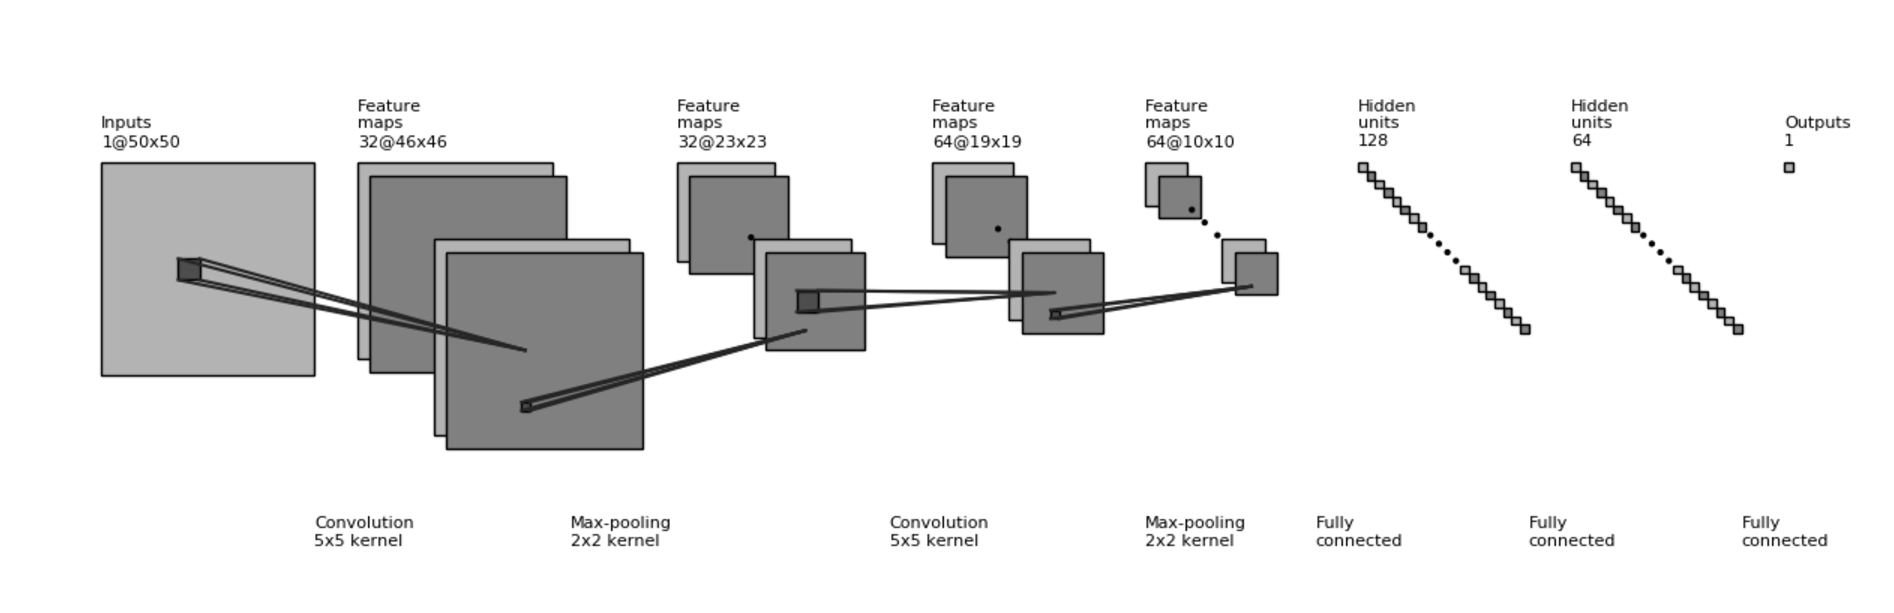
\includegraphics[scale=0.5]{eps/lenet.eps}}
    \caption{LeNet网络结构示意}
    \label{fig:label}
\end{figure}
